In this section, we clarify the algorithm {\THESYSTEM} that analyzes the adpativity of a target program in ssa language, which consists of three auxiliary algorithms: $\mathsf{AG}$ and $\mathsf{AD}$ for generating a weighted variable-based dependency graph and $\mathsf{AP}$ to find the most weighted path in the graph. We do not show details of  $\mathsf{AP}$, it is quite standard path-finding algorithm in a weighted graph. We go through the two round example to illustrate the algorithm. Finally, we show the soundness of our algorithm with respect to the adaptivity.  


\subsection{The ideas behind the algorithm}
In consideration of the definition of adaptivity from the query-based dependency graph, our analysis whose goal is a sound upper bound on the adaptivity, is supposed to take care of paths(possible adaptivity candidates) in all the possible dependency graphs (per configuration). To this end, our algorithm aims to syntactically construct a dependency graph, in which the nodes are annotated ssa variables and the directed edges showing one annotated variable may depend on the other if there exists an edge between them. Intuitively, query requests in the query-based dependency graph is assigned to  variables that appears in the  predicted ssa-variable-based dependency graph. 

The algorithm {\THESYSTEM} estimates the adaptivity from the weighted variable-based dependency graph, whose structure is shown in Figure~\ref{fig:adaptfun}. We have a look at the structure of {\THESYSTEM}. We start with the dependency graph, represented in the form of a matrix $M$. To know which variable is associated with a query request in the matrix, an extra vector $V$ is produced in the algorithm, of the size of all estimated assigned variables in the target program $\ssa{c}$. Naturally, the first question comes to us, what is the size of the matrix $M$ and $V$, or the estimated assigned variables? To solve this,    
the analysis goes through the ssa program $\ssa{c}$ twice, estimating the assigned variables to be tracked and adding the appropriate annotation $(l,w)$, in the first time scan. Those annotated variables are collected in a global list $G$, whose size determines the size of the matrix and vector. This first scan generating $G$ is conducted by the algorithm $\mathsf{AG}$ in Figure~\ref{fig:adaptfun}, which takes the target program $\ssa{c}$ as input. The global list $G$ is fed into the second scan, which decides the size of the matrix and vector.
For example, if $G$ of size $N$, then the matrix used in the second round is of size $N \times N$, and vector of size $N$. It maintains an unique mapping from variables in $G$ to the matrix $M$ and the vector $V$. For example,  the $i$th row, $j$th column of the matrix $M[i][j] =1 $ represents the may-dependency from variable $ G[i]$ to $G[j]$, $M[i][j] =0$ means no dependency. In a similar way, $V[i]=1$ means the variable $G[i]$ is assigned to a query request. The second scan of $\ssa{c}$, implemented by the algorithm $\mathsf{AD}$, then records the may-dependency in $M$, the weight is tracked in $V$. We think variable associated with a query request of weight $1$ in the graph and others of weight $0$. After the analysis of $\mathsf{AG}$ and $\mathsf{AD}$, a ssa-variable-based weighted dependency graph is constructed. We use another auxiliary algorithm $AP$ to find the path with the most weights in the graph. Then the weight is the adaptivity $A$ {\THESYSTEM} estimates.    

\begin{figure}
    \centering
    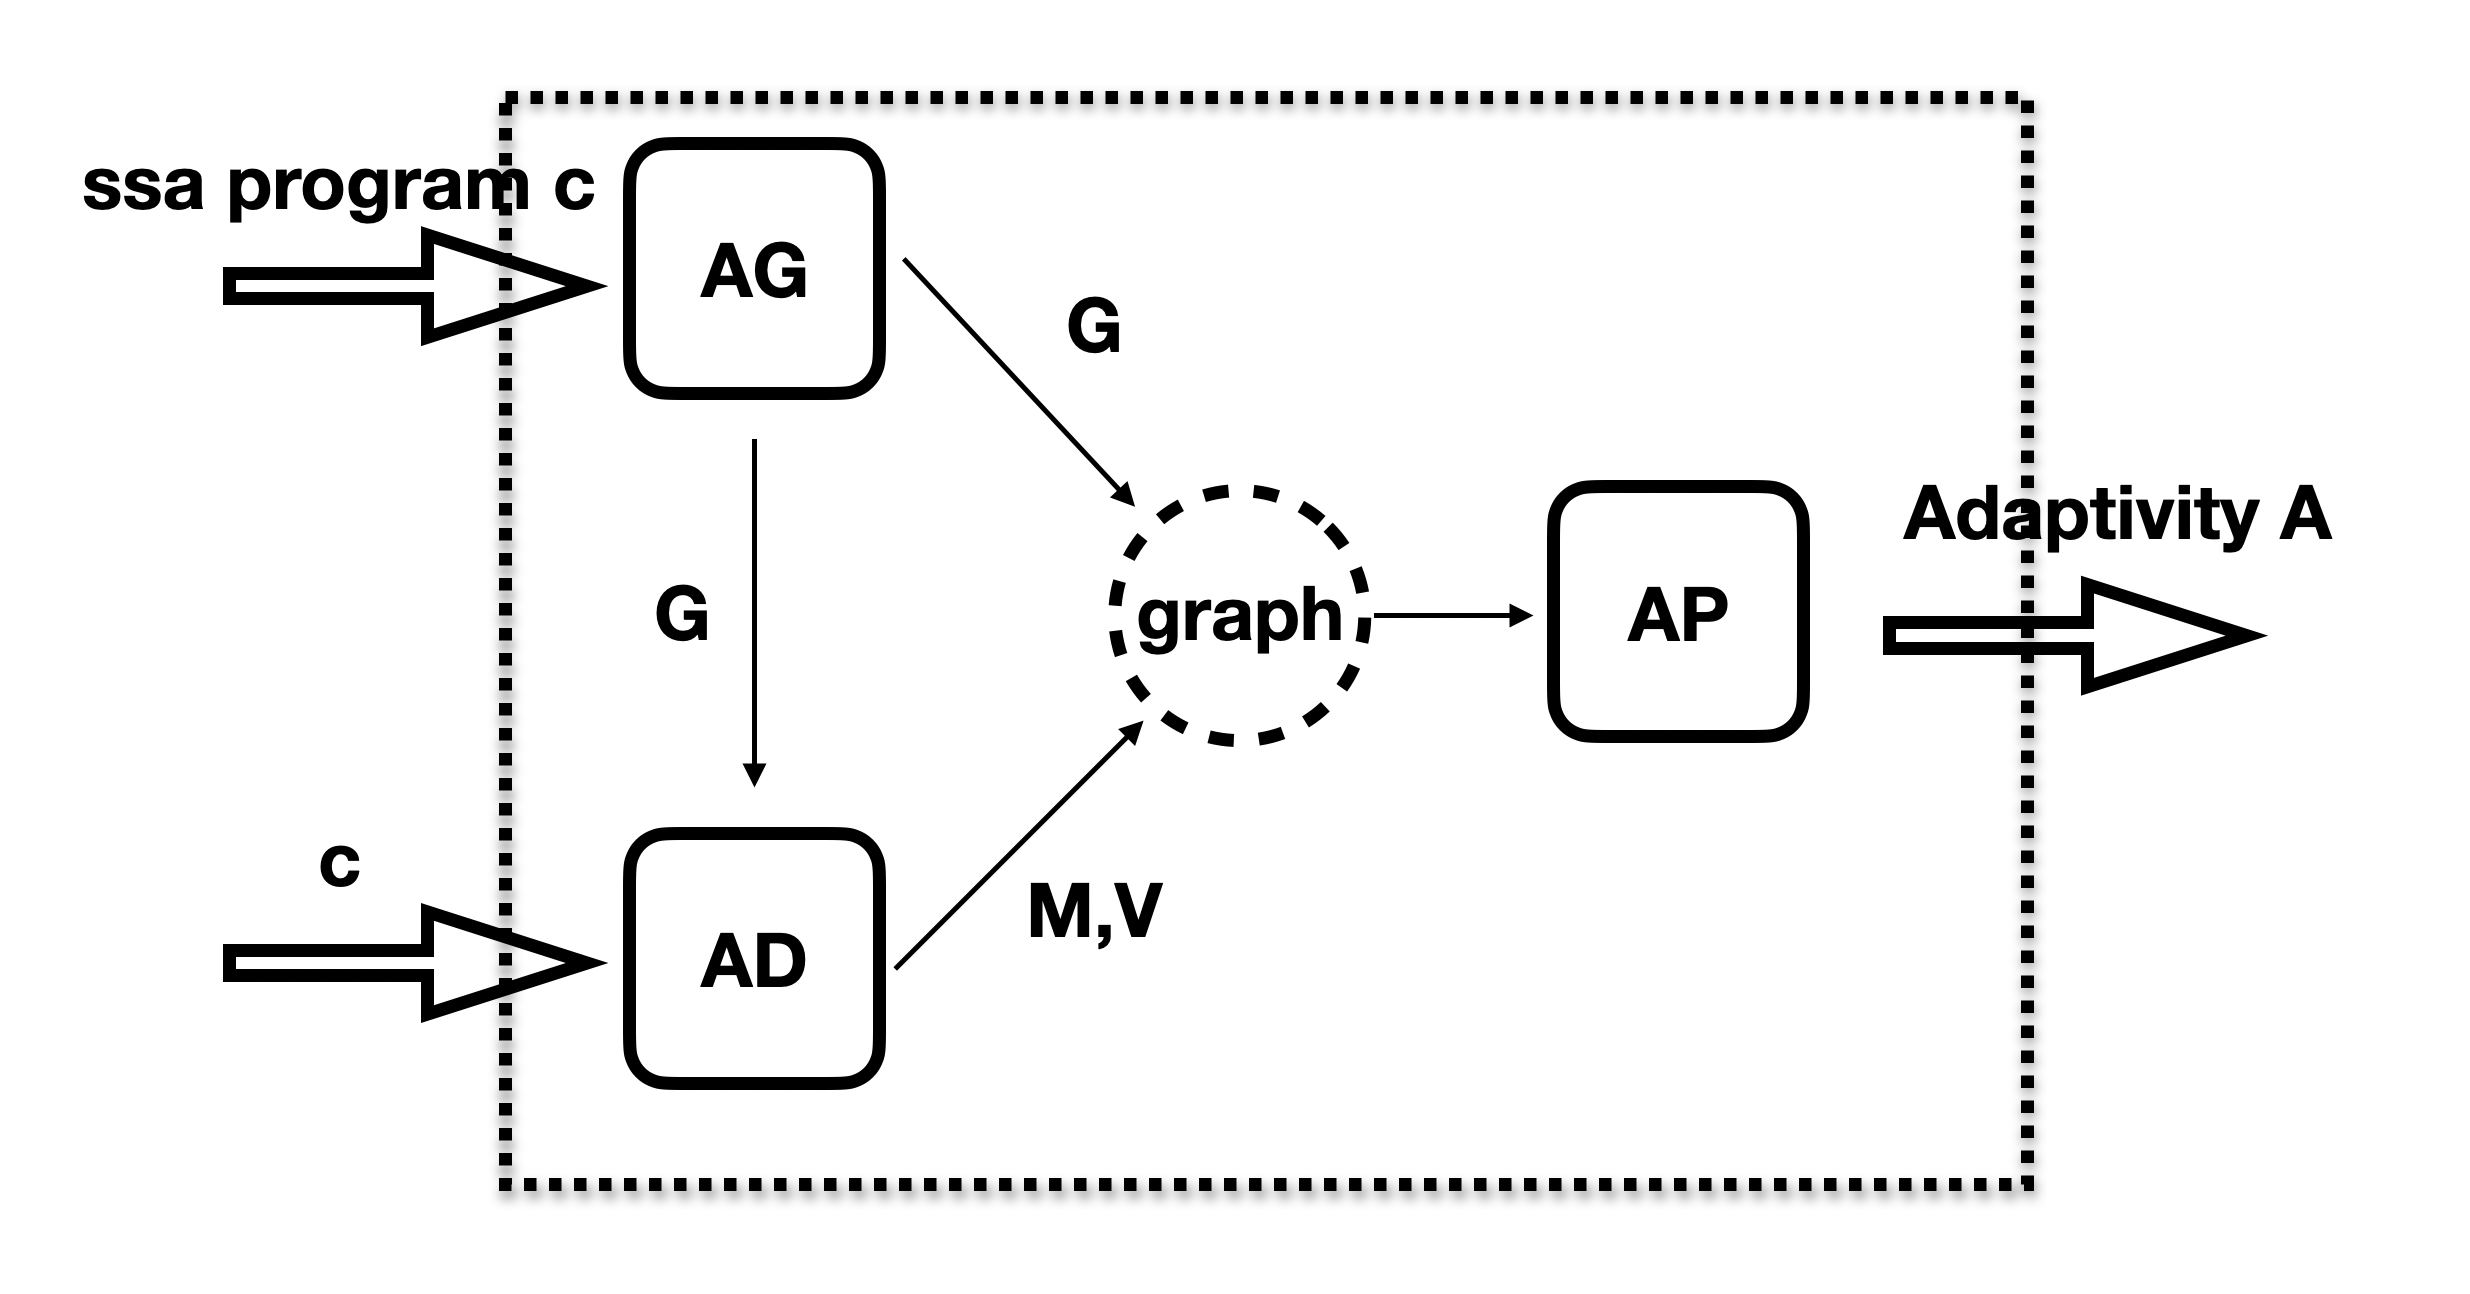
\includegraphics[width=0.7\columnwidth]{adapfun.png}
    \caption{The overview of {\THESYSTEM}}
    \label{fig:adaptfun}
\end{figure}


\subsection{Variable Estimation algorithm}
We first show how $G$ will be collected, through a variable estimating algorithm $\mathsf{AG}$ of the form $\ag{G; w; \ssa{c}}{ G'; w'} $ in Figure~\ref{fig:ag}. The input of $\mathsf{AG}$ is a list of estimated annotated variables $G$ collected before the program $\ssa{c}$, a while map $w$ consistent with previous estimation, a program $\ssa{c}$. The output of the algorithm is the updated global list $G'$, along with the updated while map $w$ for later estimation.   
\begin{figure}
 \begin{mathpar}
\inferrule
{
}
{ \ag{G ;w; \ssa{[\assign {x}{\expr}]^{l}}}{G ++ [\ssa{x}^{(l,w)}];w}
% G ;w; \ssa{[\assign {x}{\expr}]^{l}} \to G ++ [x^{(l,w)}];w 
}
~\textbf{ag-asgn}
\and
\inferrule
{
}
{ \ag{G ;w;  [ \assign{\ssa{x}}{q(\ssa{\expr})}]^{l}}{  G ++ [\ssa{x}^{(l,w)}] ; w} 
}~\textbf{ag-query}
%
\and 
%
\inferrule
{
\ag{G; w; \ssa{c_1}}{  G_1;w_1}
\and 
 \ag{G_1;w ; \ssa{c_2}}{  G_2; w_2}
 \\
 {G_3 = G_2 ++ \ssa{[\bar{x}^{(l,w)}]++ \ssa{[\bar{y}^{(l,w)}]}++ \ssa{[\bar{z}^{(l,w)}]} }}
}
{
\ag{G; w;
[\eif(\ssa{\bexpr},[ \bar{\ssa{x}}, \bar{\ssa{x_1}}, \bar{\ssa{x_2}}] ,[ \bar{\ssa{y}}, \bar{\ssa{y_1}}, \bar{\ssa{y_2}}],[ \bar{\ssa{z}}, \bar{\ssa{z_1}}, \bar{\ssa{z_2}}], \ssa{ c_1, c_2)}]^{l} }{ G_3 ;w}
}~\textbf{ag-if}
%
%
%
\and 
%
\inferrule
{
\ag{G; w; \ssa{c_1}}{ G_1; w_1}
\and 
\ag{G_1;w_1; \ssa{c_2}}{ G_2; w_2}
}
{
\ag{G; w;
\ssa{(c_1 ; c_2)}}{  G_2 ; w_2}
}
~\textbf{ag-seq}
\and 
\inferrule
{
{G_0 = G \quad w_0 =w }
\and
\forall 0 \leq z < N. 
{ \ag{ G_z ++ \ssa{[\bar{x}^{(l, {w_z}+l)}]} ; (w_z+l); \ssa{c}}{ G_{z+1} ; w_{z+1}}  }
\\
{G_f = G_N ++ \ssa{[\bar{x}^{(l, w_N \setminus l)}]} }
\and
{ \ssa{\aexpr} =  {N}  }
}
{\ag{G; w; [\eloop ~ \ssa{\aexpr}, n, [\bar{\ssa{x}}, \bar{\ssa{x_1}}, \bar{\ssa{x_2}}] ~ \edo ~ \ssa{c}]^{l} }{ G_f; w_N\setminus l }
}~\textbf{ag-loop}
% \and 
% \inferrule
% {
% \Gamma \vdash^{(i,i+a )}_{M, V} c 
% }
% {\Gamma \vdash^{(i, i+ N*a)}_{M_{i,a}^N(f), V_{i, a}^N} 
% \ewhile([\bexpr]^l,   c) : \phi \Rightarrow \psi
% }~\textbf{while}
% %
% \and
% %
% \inferrule
% {
% }
% { \ag{ G;w; [ \eswitch(\ssa{\expr}, \ssa{x},(\ssa{v_j} \rightarrow \ssa{q_j} ) )]^{l} } { G ++ [\ssa{x}^{(l, w)}] ; w} }
% ~\textbf{switch}
\end{mathpar}
 \caption{The algorithm $\mathsf{AG}$ }
    \label{fig:ag}
\end{figure}
The assignment is the source of variables $\mathsf{AG}$ estimates, in the case $\textbf{ag-asgn}$ and $\textbf{ag-query}$, the output global list is extended by $\ssa{x}^{(l,w)}$. When it comes to the if command in the rule $\textbf{ag-if}$, variables assigned in the then branch $\ssa{c_1}$, as well as the variables assigned in the else branch $\ssa{c_2}$, and the new generated variables $\bar{\ssa{x}},\bar{\ssa{y}},\bar{\ssa{z}}$ in $ [ \bar{\ssa{x}}, \bar{\ssa{x_1}}, \bar{\ssa{x_2}}] ,[ \bar{\ssa{y}}, \bar{\ssa{y_1}}, \bar{\ssa{y_2}}],[ \bar{\ssa{z}}, \bar{\ssa{z_1}}, \bar{\ssa{z_2}}]$. The sequence is standard by accumulating the predicted variables in the two commands $\ssa{c_1}$ and $\ssa{c_2}$ in a sequence $\ssa{c_1;c_2}$. The loop considers the loop iterations as well by assuming the loop counter $\ssa{\aexpr}$ to be certain natural number $N$ in the rule $\textbf{ag-loop}$. The algorithm counts the assigned variables in every iteration, including those new assigned variables in $\bar{\ssa{x}}$, those variables assigned in the body $\ssa{c}$, with the appropriate annotation showing the iteration number of the variables.      


\subsection{Matrix and Vector based algorithm}
We have a global list $G$ after the first scan of the ssa programs $\ssa{c}$. We develop a matrix and vector based approach based on the global list $G$ to get an estimated upper bound on the adaptivity of the program.  In this approach, a matrix is constructed according to those estimated annotated variables from the global list, in which every row and every column corresponds to the unique variable in $G$ by position. To be precise, in this matrix, $0$ means no dependency while non-zero value in the matrix shows may-dependency between corresponding variables. If the value of $M[i][j]$ in the matrix $M$ is greater than zero, we know annotated variable $G[i]$ may depend on $G[j]$. A vector $V$ has the same size as $G$ and it records whether the corresponding variable $G[i]$ is assigned with a query request. $V[i] =1$ means assigned with a query request and  otherwise $V[i]=0$. We call this algorithm which tracks may-dependency in the ssa programs and query information, $\mathsf{AD}$. The algorithm of the form $ \ad{\Gamma; \ssa{c} ;i }{ M; V;  i' } $, the input is a tuple consisting of three elements: (1) a one-row-N-column matrix $\Gamma$ storing the dependency from previous program, it is used when handling the if command. (2) the ssa program $\ssa{c}$ to be analyzed (3) an index $i$ specifying the location of the first assigned variable of the program $\ssa{c}$ in the global list $G$. The output of $\mathsf{AD}$ also consists of three elements ; (1) A matrix $M$ showing the may-dependency in $\ssa{c}$ (2) A vector $V$ records the query requests in $\ssa{c}$ (3) the index $i'$ that refers to the next position of the last assigned variable in $\ssa{c}$, if exists. The existence of the index $i'$ helps to locate the first assigned variable if we need to analyze programs after $\ssa{c}$.  

We first define some functions which use the indices in $G$. 
The function $\mathsf{L(i)}$ generates one-column-N-rows  matrix, where only the $i-th$ row is $1$ and all the other rows are $0$. This function is used to locate the right row when calculate the matrix when analyzing assignment and query. 

The function $\mathsf{R(e, i)}$ generates a one-row-N-column matrix. For every variable used in $e$, it finds the corresponding index $i$ in $G$ so that $G[i]$ maps to the variable and mark the $i$th column as $1$. If it is not found, we do not mark. When we say $G[i]$ maps to a target variable, we take off the annotation of $G[i]$ and check if the left variable is the same as the target variable. To handle loop, for instance, a variable $y$ appears many times in $G$, but with different annotations(iteration numbers), the argument $i$ helps to find most recent assignment variable $y$ before the index $i$ in $G$. It is still used when analyzing assignment and query. Thanks to our ssa language, our choice of the most recent assigned variable is reasonable because the variable used in the loop refers to the most recent assignment and every variable is uniquely assigned in its ssa form. 

We define $M_1;M_2$ to combine two matrix, where $M_1 + M_2$ is the standard sum of two matrix.
\[
M_1 ; M_2  :=  M_2 \cdot M_1 + M_1 + M_2 
\]
And define the operator $\uplus$ to combine two vectors.
\[
V_1 \uplus V_2  :=  \left\{
\begin{array}{ll}
1 & (V_1[i] = 1 \lor V_2[i] = 1) \land i = 1, \cdots, N \land |V_1| = |V_2|\\
0 & o.w.
\end{array}\right.
\]
For the sake of brevity, we also define some annotations as follows. We show how the algorithm $\mathsf{AD}$ handles the extra part $[ \bar{\ssa{x}}, \bar{\ssa{x_1}},\bar{\ssa{x_2}} ] $ in the if and loop commands. First, we give a unique name for variables in lists $\bar{\ssa{x}}, \bar{\ssa{x_1}}, \bar{\ssa{x_2}}$ respectively, as follows: {$ \forall 0 \leq z < |\bar{\ssa{x}}|. \bar{\ssa{x}}(z) = \ssa{x_z}, \bar{\ssa{x_1}}(z) = \ssa{x_{1z}}, \bar{\ssa{x_2}}(z) = \ssa{x_{2z}} $ }. And then we treat every tuple $(\ssa{x_z},\ssa{x_{1z}},\ssa{x_{2z}} )$ in $[\bar{\ssa{x}}, \bar{\ssa{x_1}}, \bar{\ssa{x_2}} ]$ as the simple may dependency case : $\ssa{x_z}$ may depend on both $ \ssa{x_{1z}}$ and $\ssa{x_{2z}}$, just like $ \assign{\ssa{x_z} }{\ssa{x_{1z}} + \ssa{x_{2z}} }$, defined as follows. 
$
 \ad{\Gamma; [\bar{\ssa{x}}, \bar{\ssa{x_1}}, \bar{\ssa{x_2}} ] ; i }{ M; V_{\emptyset}; i + |\bar{\ssa{x}}| } 
  \triangleq { \forall 0 \leq z < |\bar{\ssa{x}}|.
  \ad{\Gamma;\assign{\ssa{x_z} }{\ssa{x_{1z}} + \ssa{x_{2z}} }; i+z }{ M_{x_z};  V_{\emptyset}; i+z+1} }$
   where $M = \sum_{o \leq z < |\bar{\ssa{x}}| }M_{x_z} $.
% \framebox{$ \ad{\Gamma; \ssa{c} ; i_1){M;V;i_2} $}
%
\begin{figure}
\begin{mathpar}
\inferrule
{M = \mathsf{L}(i) * ( \mathsf{R}(\ssa{\expr},i) + \Gamma )
}
{
 \ad{\Gamma;[\assign {\ssa{x}}{\ssa{\expr}} ]^{l}; i }{M; V_{\emptyset}; i+1 }
% \Gamma \vdash_{M, V_{\emptyset}}^{(i, i+1)} [\assign {\ssa{x}}{\ssa{\expr}} ]^{l}
}
~\textbf{ad-asgn}
\and
\inferrule
{M = \mathsf{L}(i) * ( \mathsf{R}(\ssa{\expr},i) + \Gamma )
\\
V= \mathsf{L}(i)
}
{ 
\ad{\Gamma;[ \assign{\ssa{x}}{q(\ssa{\expr})} ]^{l} ; i }{M;V;i+1}
%  \vdash^{(i, i+1)}_{M, V} [ \assign{\ssa{x}}{q(\ssa{\expr})} ]^{l} 
}~\textbf{ad-query}
%
\and 
%
\inferrule
{
{\ad{\Gamma + \mathsf{R}(\ssa{\bexpr}, i_1); \ssa{c_1} ; i_1 }{ M_1;V_1;i_2 }}
% \Gamma + \mathsf{R}(\bexpr, i_1) \vdash^{(i_1, i_2)}_{M_1, V_1} \ssa{c_1} 
% : \Phi \land \bexpr \Rightarrow \Psi
\and 
{\ad{\Gamma + \mathsf{R}(\ssa{\bexpr}, i_1);\ssa{c_2} ; i_2 }{ M_2; V_2 ;i_3}}
% \Gamma + \mathsf{R}(\ssa{\bexpr}, i_1) \vdash^{(i_2, i_3)}_{M_2, V_2} \ssa{c_2} 
% : \Phi \land \neg \bexpr \Rightarrow \Psi
\\
% { \forall 0 \leq j < |\bar{x}|. \bar{x}(j) = x_j, \bar{x_1}(j) = x_{1j}, \bar{x_2}(j) = x_{2j}  }
{\ad{\Gamma; [ \bar{\ssa{x}}, \bar{\ssa{x_1}}, \bar{\ssa{x_2}}]; i_3 }{ M_x; V_{\emptyset}; i_3+|\bar{\ssa{x}}| }}
%
\and
%
{\ad{\Gamma; [ \bar{\ssa{y}}, \bar{\ssa{y_1}}, \bar{\ssa{y_2}}]; i_3+|\bar{\ssa{x}}| }{ M_y; V_{\emptyset}; i_3+|\bar{\ssa{x}}|+|\bar{\ssa{y}}| }}
%
\\
%
{\ad{\Gamma; [ \bar{\ssa{z}}, \bar{\ssa{z_1}}, \bar{\ssa{z_2}}]; i_3+|\bar{\ssa{x}}|+ |\bar{\ssa{y}}|}{ M_y; V_{\emptyset}; i_3+|\bar{\ssa{x}}|+|\bar{\ssa{y}}| + |\bar{\ssa{z}}| }}
% { \forall 0 \leq j < |\bar{x}|.  \Gamma \vdash_{M_{x_j}, V_{\emptyset}}^{i_3+j, i_3+j+1 } x_j \leftarrow x_{1j} + x_{2j} }
% \and
% { \forall 0 \leq j < |\bar{y}|.  \Gamma \vdash_{M_{y_j}, V_{\emptyset}}^{i_3+|\bar{x}|+j, i_3+|\bar{x}|+j+1 } y_j \leftarrow y_{1j} + y_{2j} }
% \\
% { \forall 0 \leq j < |\bar{z}|.  \Gamma \vdash_{M_{z_j}, V_{\emptyset}}^{i_3+|\bar{x}|+|\bar{y}|+j, i_3+|\bar{x}|+|\bar{y}|+j+1 } z_j \leftarrow z_{1j} + z_{2j} }
\\
{M = (M_1+M_2)+ M_x+M_y +M_z }
}
{
\Gamma \vdash^{(i_1, i_3+|\bar{x}|+|\bar{y}|+|\bar{z}|)}_{M, V_1 \uplus V_2 } 
[\eif(\ssa{\bexpr},[ \bar{\ssa{x}}, \bar{\ssa{x_1}}, \bar{\ssa{x_2}}] ,[ \bar{\ssa{y}}, \bar{\ssa{y_1}}, \bar{\ssa{y_2}}] , [ \bar{\ssa{z}}, \bar{\ssa{z_1}}, \bar{\ssa{z_2}}] , \ssa{ c_1, c_2)}]^{l}
}~\textbf{ad-if}
%
%
%
\and 
%
\inferrule
{
{\ad{\Gamma; \ssa{c_1} ; i_1 }{ M_1 ; V_1; i_2 }  }
% \Gamma \vdash^{(i_1, i_2)}_{M_1, V_1} \ssa{c_1} 
% : \Phi \Rightarrow \Phi_1
\and 
{\ad{\Gamma;\ssa{c_2}; i_2}{M_2; V_2 ;i_3 }}
% \Gamma \vdash^{(i_2, i_3)}_{M_2, V_2} \ssa{c_2} 
% : \Phi_1 \Rightarrow \Psi 
}
{
\ad{\Gamma ; (\ssa{c_1 ; c_2} ) ; i_1}{(M_1 {;} M_2) ; V_1 \uplus V_2 ; i_3  }
% \Gamma \vdash^{(i_1, i_3)}_{M_1 {;} M_2, V_1 \uplus V_2}
% \ssa{c_1 ; c_2} 
% : \Phi \Rightarrow \Psi
}
~\textbf{ad-seq}
\and 
\inferrule
{
B= |\ssa{\bar{x}}| \and {A = |\ssa{c}|}
% \and
% {\Gamma \vdash^{(i, i+B)}_{M_{10}, V_{10}} [\bar{\ssa{x}}, \bar{\ssa{x_1}}, \bar{\ssa{x_2}}] }
% \and
% {\Gamma \vdash^{(i+B,i+B+A )}_{M_{20}, V_{20}} \ssa{c} 
% }
\\
\forall 0 \leq j < N. 
{\ad{\Gamma;[\bar{\ssa{x}}, \bar{\ssa{x_1}}, \bar{\ssa{x_2}}]; i+ j*(B+A) }{M_{1j};V_{1j}; i+B+j*(B+A) }}
% {\Gamma \vdash^{(i+j*(B+A), i+B+j*(B+A))}_{M_{1j}, V_{1j}}  } [\bar{\ssa{x}}, \bar{\ssa{x_1}}, \bar{\ssa{x_2}}]
\\
{
\ad{\Gamma;\ssa{c} ; i+B+j*(B+A)  }{M_{2j}; V_{2j}; i+B+A+j*(B+A) }
% \Gamma \vdash^{(i+B+j*(B+A),i+B+A+j*(B+A) )}_{M_{2j}, V_{2j}} \ssa{c} 
% : \Phi \land e_n = \lceil{z+1}\rceil \Rightarrow \Psi 
}
\\
{
\ad{\Gamma ; [\bar{\ssa{x}}, \bar{\ssa{x_1}}, \bar{\ssa{x_2}}] ; i+N*(B+A) }{M; V ;i+N*(B+A)+B}
% \Gamma \vdash^{(i+N*(B+A) ,i+N*(B+A)+B )}_{M, V} [\bar{\ssa{x}}, \bar{\ssa{x_1}}, \bar{\ssa{x_2}}]
% : \Psi \Rightarrow \Phi \land e_N = \lceil{z}\rceil 
}
\\
{ \ssa{\aexpr} =  {N}  }
\and
{M' = M+ \sum_{0 \leq j <N}( M_{1j}+M_{2j})  }
\and
{V' = V \uplus \sum_{0 \leq j <N}( V_{1j} \uplus V_{2j})  }
}
{\Gamma \vdash^{(i, i+N*(B+A)+B   )}_{M', V'} 
[\eloop ~ \ssa{\aexpr}, 0, [\bar{\ssa{x}}, \bar{\ssa{x_1}}, \bar{\ssa{x_2}}] ~ \edo ~ \ssa{c}]^{l}
% : \Phi \land \expr_N = \lceil { N} \rceil \Rightarrow \Phi \land \expr_N = \lceil{0}\rceil
}~\textbf{ad-loop}
% \and 
% \inferrule
% {
% \Gamma \vdash^{(i,i+a )}_{M, V} c 
% }
% {\Gamma \vdash^{(i, i+ N*a)}_{M_{i,a}^N(f), V_{i, a}^N} 
% \ewhile([\bexpr]^l,   c) : \phi \Rightarrow \psi
% }~\textbf{while}
% %
% \and
% %
% \inferrule
% { \Gamma + \mathsf{R}(\expr,i) \vdash^{(i, i+1)}_{M, V} \assign{ x}{q_j} 
% % : \Phi \Rightarrow \Psi
% \\
% j \in \{1, \dots, N\}     }
% {\Gamma \vdash^{(i, i+1)}_{ M,V } 
% [\eswitch(\ssa{\expr}, \ssa{x},(v_j \rightarrow q_j ) ]^{l}
% % : \Phi \Rightarrow \Psi 
% }
% ~\textbf{switch}
% %
% \and
% %
% \inferrule
% { 
% \vDash 
% \Phi \Rightarrow \Phi'  
% \and
% \Gamma \vdash^{(i_1, i_2)}_{(M',V')} c : \Phi' \Rightarrow \Psi'
% \and
% \vDash \Psi' \Rightarrow \Psi
% \and 
% \Phi \vDash M' \leq M
% \and 
% \Phi \vDash V' \leq V
% }
% {\Gamma \vdash^{(i_1, i_2)}_{(M,V)} c 
% : \Phi \Rightarrow \Psi
% }
% ~\textbf{conseq}
\end{mathpar}
    \caption{The algorithm AD}
    \label{fig:algo_ad}
\end{figure}
One of the key idea under algorithm $\mathsf{AD}$ is to track the indices $i$,$i'$ both in the input and output to synchronize with its previous algorithm $\mathsf{AG}$. The index in $\mathsf{AD}$ increases as the same way as the global list expands after the analysis of a program $\ssa{c}$, which helps $\mathsf{AD}$ record the dependency relation from the program $\ssa{c}$ in the right place of the matrix. For example, in the case $\textbf{ad-asgn}$ and $\textbf{ad-query}$, the index increases by 1, which corresponds to their counterparts of algorithm $\textbf{AG}$. The if and loop commands have the extra part $ [\bar{\ssa{x}}, \bar{\ssa{x_1}}, \bar{\ssa{x_2}}] $ and we find that the output index increases by also considering this part as we do in collecting the global list.  

Another interesting point is the construction of the matrix. The fundamental case is the assignment and query cases. We use a function $L(i)$ to generate a N-row-one-column matrix $L$ to guarantee the resulting matrix only has non-zeros at row $i$. The intuition behind is that one single assignment or query request can only reveal the dependency of its assigned variable (corresponding to one row of the matrix) to the variables used on the right hand sides. Thanks to the index $i$, we know which row this assignment should be in the matrix. The function $\mathsf{R}(\ssa{\expr},i)$ gets a one-row-N-column matrix marking the variables used in the right hand side. The $\Gamma$ is designed for the if command and we will discuss it later. We can see one simple example $sa$ to get a taste.     
\[
sa \triangleq
\begin{array}{l}
    \left[x_1 \leftarrow 2 \right]^1; \\
    \left[x_2 \leftarrow x_1 + 2 \right]^2 ; \\
    \left[x_3 \leftarrow x_1 + x_2 \right]^3
\end{array}
\]
In the program $sa$, only simple assignment is involved. When we assume $\Gamma$ is empty, for the assignment at line $3$, the matrix is built as follows.
\[
\textbf{line3:} ~~
 \left[x_3 \leftarrow x_1 + x_2 \right]^3 :
 ~~~
\begin{blockarray}{cc}
\begin{block}{c[c]}
 x_1 & 0   \\
 x_2 & 0 \\
 x_3 & 1 \\
\end{block}
\end{blockarray}
*
\begin{blockarray}{ccc}
x_1 & x_2 & x_3 \\
\begin{block}{[ccc]}
1 & 1 & 0 \\
\end{block}
\end{blockarray}
= 
\begin{blockarray}{cccc}
& x_1 & x_2 & x_3\\
\begin{block}{c[ccc]}
x_1 & 0 & 0 & 0 \\
x_2 & 1 & 0 & 0 \\
x_3 & 1 & 1 & 0 \\
\end{block}
\end{blockarray}
\]
% a simple example of assignment
% \begin{example}[Simple Assignment]
% \[
% SA \triangleq
% \begin{array}{l}
%     \left[x_1 \leftarrow 2 \right]^1; \\
%     \left[x_2 \leftarrow x_1 + 2 \right]^2 ; \\
%     \left[x_3 \leftarrow x_1 + x_2 \right]^3
% \end{array}
% \]
% %
% %
% \[
%  \textbf{line2:} ~~
%  \left[x_2 \leftarrow x_1 + 2 \right]^2 :
%  ~~~
% \begin{blockarray}{cc}
% \begin{block}{c[c]}
%  x_1 & 0   \\
%  x_2 & 1 \\
%  x_3 & 0 \\
% \end{block}
% \end{blockarray}
% *
% \begin{blockarray}{ccc}
% x_1 & x_2 & x_3 \\
% \begin{block}{[ccc]}
% 1 & 0 & 0 \\
% \end{block}
% \end{blockarray}
% = 
% \begin{blockarray}{cccc}
% & x_1 & x_2 & x_3\\
% \begin{block}{c[ccc]}
% x_1 & 0 & 0 & 0 \\
% x_2 & 1 & 0 & 0 \\
% x_3 & 0 & 0 & 0 \\
% \end{block}
% \end{blockarray}
% \]
% %
% %
% %
% \[
% \textbf{line3:} ~~
%  \left[x_3 \leftarrow x_1 + x_2 \right]^3 :
%  ~~~
% \begin{blockarray}{cc}
% \begin{block}{c[c]}
%  x_1 & 0   \\
%  x_2 & 0 \\
%  x_3 & 1 \\
% \end{block}
% \end{blockarray}
% *
% \begin{blockarray}{ccc}
% x_1 & x_2 & x_3 \\
% \begin{block}{[ccc]}
% 1 & 1 & 0 \\
% \end{block}
% \end{blockarray}
% = 
% \begin{blockarray}{cccc}
% & x_1 & x_2 & x_3\\
% \begin{block}{c[ccc]}
% x_1 & 0 & 0 & 0 \\
% x_2 & 1 & 0 & 0 \\
% x_3 & 1 & 1 & 0 \\
% \end{block}
% \end{blockarray}
% \]
% %
% \end{example}
 We use a one-row-N-column matrix $\Gamma$ as one of the input of $\mathsf{AD}$, to handle the cases when the control flow diverges in the labelled if command $[\eif(\ssa{\bexpr},[ \bar{\ssa{x}}, \bar{\ssa{x_1}}, \bar{\ssa{x_2}}] ,[ \bar{\ssa{y}}, \bar{\ssa{y_1}}, \bar{\ssa{y_2}}] , [ \bar{\ssa{z}}, \bar{\ssa{z_1}}, \bar{\ssa{z_2}}] , \ssa{ c_1, c_2)}]^{l} $, where the execution of either branch may depend on the conditional guard $\ssa{\bexpr}$. Follow this intuition, the analysis of either branch is supposed to consider the variables used in the conditional $\ssa{\bexpr}$, tracked in $\Gamma$. In the case $\textbf{ad-if}$, we can see the analysis of the two branches $\ssa{c_1}$ and $\ssa{c_2}$ share the same input $\Gamma + \mathsf{R}(\ssa{\bexpr}, i)$ and $\mathsf{R}(\ssa{\bexpr}, i) $ tells the variables assigned before the if command and used in the conditional $\ssa{\bexpr}$.   

We compose the matrix and vectors in the case of sequence in $\textbf{ad-seq}$. The non-zeros or we call it effect range of the matrix and vector is decided by its input and output indices. From the case $\textbf{ad-seq}$, two programs $\ssa{c_1}$ and $\ssa{c_2}$ have disjoint effect ranges $[i_1, i_2)$ and $[i_1,i_3)$, it is safe to combine them without lose information. 

The loop case is handled in a well organized way. We use $B= |\bar{\ssa{x}}|$ and $A= |{\ssa{c}}|$ to estimate the size of variables assigned in $\bar{\ssa{x}}$ and $\ssa{c}$. And  $|\ssa{c}|$ is defined by the help of the algorithm $\mathsf{AG}$, defined as $|\ssa{c}|= |G|$ when $\ag{[];\ssa{c};\emptyset }{ G; \emptyset }$. The algorithm then gets how many iterations $N$ the loop may executes from the loop counter $\ssa{\aexpr}$. For every iteration, it first records the dependency relations between variables in $ [\bar{\ssa{x}}, \bar{\ssa{x_1}}, \bar{\ssa{x_2}}]$ by constructing a corresponding matrix $M_{1j}$ ($j$ is the iteration number) and an empty vector $V_{1j}$, and analyze the loop body $\ssa{c}$ with a resulting matrix $M_{2j}$ and vector $V_{2j}$. We give an extra analysis of those new assigned variables as what $\mathsf{AG}$ does, it works well when the loop is executed ($N = 0$) or not. We know that for all the possible iteration number $j$, $M_{1j}$ and $M_{2j}$ have disjoint effect ranges so we combine them, similar as the vectors $V_{1j}$ and $V_{2j}$.   

Finally, we are able to construct a variable-based weighted dependency graph based on $G$,$M$ and $V$ generated by the framework. The definition of the estimated adaptivity is the weight of the most weighted path in the graph defined as follows. 

\begin{defn}
[Estimated Adaptivity]
Given a program $\ssa{c}$, the global list $G$, and $\ad{\Gamma; \ssa{c}; i_1}{M, V, i_2}$, the weighted dependency graph $G_{ssa}(M, V,G,i_1,i_2) = (Nodes, Edges, Weights)$ is defined as:
\\
Nodes $Vt = \{ G(j) \in \mathcal{LV} \mid i_1 \leq j < i_2 \}$
\\
Edges $E = \{ (G(j_1), G(j_2)) \in \mathcal{LV} \times \mathcal{LV} \mid M[j_1][j_2] \geq 1 \land  i_1 \leq j_1,j_2 < i_2   \}$
\\
 Weights $Wt = \{ (  G(j), 1 ) \in \mathcal{LV} \times \mathcal{N} | i_1 \leq j < i_2 \land V[j] = 1\}
        \cup \{ (  G(j), 0 ) \in \mathcal{LV} \times \mathcal{N} | i_1 \leq j < i_2 \land V[j] = 0 \} $.
        
Adaptivity of the program defined according to the graph is as:
\[
Adapt(M, V,i_1,i_2) := \max_{vt_1, vt_2 \in Vt}\{ \mathsf{Weight}( p(vt_1, vt_2), Wt) \},
\]
where $p(k, l)$ is the path in graph $G_{ssa}(M, V, i_1,i_2)$ starting from $k$ to $l$, $\mathsf{Weight}(p(vt_1,vt_2), Wt)$ get the total sum of weights along the path $p(vt_1,vt_2)$.
\end{defn}        

\subsection{Analysis on two round algorithm}
We show how {\THESYSTEM} analyze the two round algorithm. For the sake of brevity, we conduct the analysis on the simplified two round algorithm $TR^{ssa}$.

% \[
% TR^{ssa}(k) \triangleq
% {
% \begin{array}{l}
%     % \left[j \leftarrow 0 \right]^1 ; \\
%     \clabel{a_1 \leftarrow []}^{1} ; \\
%     \clabel{\assign{j_1}{0} }^{2} ; \\
%     \eloop ~ \clabel{k}^{3} ~ \edo [(j_3, j_1,j_2),(a_3, a_1,a_2)]~ \\
%     \Big(
%     \clabel{ x_1 \leftarrow q(\chi(j_3)\cdot \chi(k))}^{4}  ; \\
%     \clabel{ \assign{j_2}{j_3+1} }^{5} ;\\
%     \clabel{a_2 \leftarrow x_1 :: a_3}^{6}       \Big);\\
%     \clabel{l_1 \leftarrow q(\mathrm{sign}\big (\sum_{i\in [k]} \chi(i)\times\ln\frac{1+a_3[i]}{1-a_3[i]} \big ))}^{7}\\
% \end{array}
% }
% \]
{\THESYSTEM} first runs the algorithm $\mathsf{AG}$ to generate the global list $G$. We assume the input $k=2$ and have the following.

\[G_{k=2} = \left[
  {a_1}^{(1,\emptyset)} , {a_3}^{(2,[2:1])} , {x_1}^{(3,[2:1])} , {a_2}^{(4,[2:1])} ,  {a_3}^{(2,[2:2])} , {x_1}^{(3,[2:2])} , {a_2}^{(4,[2:2])} , {a_3}^{(2,\emptyset)} , {l_1}^{(5,\emptyset)}   \right] \]
% \[G_{k=2} = \left[ \begin{array}{l}
%      {a_1}^{(1,\emptyset)} , {j_1}^{(2,\emptyset)}, {j_3}^{(3,[2:1])} , {a_3}^{(3,[2:1])} , {x_1}^{(4,[2:1])} ,{j_2}^{(5,[2:1])} ,
%   {a_2}^{(6,[2:1])},  \\
%     {j_3}^{(3,[2:2])} , {a_3}^{(3,[2:2])} , {x_1}^{(4,[2:2])} ,{j_2}^{(5,[2:2])} ,
%   {a_2}^{(6,[2:2])},
%   {j_3}^{(3,\emptyset)} , {a_3}^{(3,\emptyset)} ,
%   {l_1}^{(7,\emptyset)} \\  
% \end{array}
%      \right] \]
 We denote $a_1^{1}$ short for ${a_1}^{(1,\emptyset)}$ and ${a_3}^{(2,1)}$ short for ${a_3}^{(2,[2:1])}$. Then the resulting matrix $M_{tr}$ and $V_{tr}$ of the algorithm $\mathsf{AD}$ as follows.
 
{ \tiny
 \[
M_{tr} =  \left[ \begin{matrix}
 & a_1^{1} & a_3^{(2,1)} & x_1^{(3,1)} & a_2^{(4,1)}  & a_3^{(2,2)} & x_1^{(3,2)} & a_2^{(4,2)} & a_3^{2} & l_1^{5}\\
 a_1^{1} & 0 & 0 & 0 & 0 & 0 & 0 & 0 &0 &0 \\
a_3^{(2,1)} & 1 & 0 & 0 & 0 & 0 & 0 & 0&0&0\\
x_1^{(3,1)} & 0 & 0 & 0 & 0 & 0 & 0& 0& 0 &0\\
a_2^{(4,1)} & 0 & 1 & 1 & 0 & 0 & 0 & 0& 0&0\\
a_3^{(2,2)} & 1 & 0 & 0 & 1 & 0 & 0 & 0 & 0&0 \\
x_1^{(3,2)} & 0 & 0 & 0 & 0 & 0 & 0 & 0& 0&0\\
a_2^{(4,2)} & 0 & 0 & 0 & 0 & 1 & 1 & 0& 0&0\\
a_3^{2} & 1 & 0 & 0 & 0 & 0 & 0 & 1& 0&0\\
l_1^{5} & 0 & 0 & 0 & 0 & 0 & 0 & 0 & 1 &0 \\
 \end{matrix} \right] 
~ , V_{tr} = \left [ \begin{matrix}
a_1^{1} &  0 \\
a_3^{(2,1)} & 0 \\
x_1^{(3,1)} & 1 \\
a_2^{(4,1)} &  0 \\
a_3^{(2,2)} & 0 \\
x_1^{(3,2)} & 1 \\
a_2^{(4,2)} &  0 \\
a_3^{2} &  0 \\
l_1^{5} &  1 \\
\end{matrix} \right ]
\]
}
%% a graph is better here

\subsection{ Soundness of {\THESYSTEM}}
We would like to show that the query-based dependency graph generated from the trace of the execution of the target ssa program is a subgraph of the variable-based dependency graph predicted from our algorithm ${\THESYSTEM}$, and the query requested during the execution is also bounded by an estimation from our algorithm.

We first give a definition of subgraph of a query-based dependency graph with respect to a variable-based dependency graph.
\begin{defn}
[Subgraph]
Given a query-based dependency graph $G_{s} = (V_1, E_1)$, a variable-based dependency graph $G_{ssa} = (V_2, E_2)$, $G_{s} \subseteq G_{ssa}$ iff:\\
$\exists f$ so that \\
1. for every $v \in V_1$, $f(v) \in V_2$. 
\\
2. $\forall e=(v_i, v_j) \in E_1$, there exists a path 
% $g(e)$ 
from $f(v_i)$ to $f(v_2)$ in $G_{ssa}$.
\end{defn}

Then we show the soundness of {\THESYSTEM}. In the theorem, we use some definition. $G \vDash M, V$ says that $G$ and $M$, $V$ have the corresponding size. $G; w \vDash (\ssa{c}, i_1,i_2)$ checks if the variables assigned in $\ssa{c}$ calculated by $\mathsf{AG}$ matches the variables in $G$ from index $i_1$ to $i_2$.

\begin{thm}
[Soundness of {\THESYSTEM}]
Given $ \ad{\Gamma; \ssa{c}; i_1 }{M; V;i_2}$,  for any global list $G$,  loop maps $w$ such that $G ;w \vDash (\ssa{c}, i_1, i_2) \land G \vDash (M,V)$. $K$ is the number of queries inquired during the execution of the piece of program $\ssa{c}$ and |V| gives the number of non-zeros in $V$. 
% $|.|_{low} $ is the annotation erasure, which turns a ssa form program $\ssa{c}$ to its low-level version.
Then,
\[
K \leq |V| \land \forall D, \ssa{m}. G_{s}(\ssa{c},D,\ssa{m},w) \subseteq G_{ssa}(M, V,G,i_1, i_2)
\]      
\end{thm}
